\documentclass[11pt,a4paper]{article}
\usepackage[utf8]{inputenc}
\usepackage{ctex}
\usepackage{amsmath,amssymb,amsfonts,amsthm}
\usepackage{graphicx}
\usepackage{hyperref}
\usepackage{booktabs}
\usepackage{geometry}
\geometry{left=2.5cm,right=2.5cm,top=3cm,bottom=3cm}

\title{\textbf{全息抗熵理论：开放复杂巨系统的形式化证明、可计算重塑与碳硅共生自愈演化}}
\author{\textbf{作者}：孟凡淳（Grit Meng）¹ \\ \small ¹ 全域数字神经中枢总体设计部}
\date{\today}

\begin{document}
\maketitle

\begin{abstract}
面对现代开放复杂巨系统（OCGS）呈现的非独立同分布（Non-IID）及阶乘级状态空间大爆炸，传统的还原论解析方案与基于静态稳态假设的开环观测器已深陷耗散死锁。本文正式阐明全息抗熵理论（Holographic Anti-Entropy, HAE）的普适科学范式，在统计物理、控制论、测度论与拓扑代数的最深处，确立了系统的四重断代法理主权：
“立宪”首次在工程与数学层面，系统性完成了对钱学森先生“开放复杂巨系统”与“从定性到定量综合集成方法”理论的形式化重构与判决性实证，验证了其学说的绝对正确性，确立了由五维正交时空容器 $D$ 与离散时间算法引擎 $A$ 深度耦合而成的数字双螺旋本体 $\langle D, A \rangle$，定义了“综合集成是机制论，人机协同是本质论”的最高科学立宪；
“封疆”将控制论域从局部人治系统，沿变分自由能最小化轨线，向无机自组织与有机活跃群落执行尺度的分形同构延拓，确立了普适大一统状态演化方程；
“铸剑”针对“计算不可约性”与高维涌现死锁，发展出基于物理极值约束代数截断的强力剪枝法则，通过去语义化面向数据设计与二进制位图向量化，在个人笔记本上实现了5分钟内全盘收敛并刚性反写50万笔订单、20层纠缠、200万物料大盘的有限产能决策的判决性物理实证；
“选帅”首次从神经科学与自适应控制层面，系统性地构建并定义了驾驭复杂巨系统的总设计师之 L0 级底层认知操作系统（良知、高敏感、极度感性、强元认知与流体智力），解开了符号接地难题，为国家级领军人才土壤的改良提供了刚性判词。
\end{abstract}

\textbf{关键词}：全息抗熵；开放复杂巨系统；数字双螺旋本体；计算不可约性；碳硅拓扑共生；L0级底层操作系统；钱学森学派

\newpage

\section{引言：还原论的极限与系统科学的物理立宪}

经典物理学与早期系统工程在面对局部、稳态且满足独立同分布假设的简单系统时，展现出了极高的还原论定性与定量精度。然而，当科学观测的视角推移至现代数字工业网络、宏观经济体及生物活性流体等开放复杂巨系统（Open Complex Giant System, OCGS）时，系统的成分维数与交互关系呈现出强烈的非独立同分布及阶乘级组合爆炸。

根据热力学第二定律，任何孤立系统的熵在时间轴上必然自发递增，系统的自然演化终局是彻底的无序热寂与解体。在面对此种巨系统的无情耗散时，经典管理学与硅基 AGI 的纯概率派研究者本能地陷入了双重死锁：
\begin{enumerate}
    \item \textbf{人治协同的内耗内爆}：由于人脑处理并发信息的生理带宽受限于米勒极限，传统组织试图通过行政指令、线性流程拼接与无向的“跨部门民主拉通会”来平铺高维复杂性。这不仅无法在多目标约束冲突下求得全局最优，反而导致信息信道在跨层级传播时剧烈衰减，沟通通道呈平方级摩擦爆炸，产生天量的组织热耗散，使系统无可挽回地死锁在低效的纳什均衡耗散稳态中；
    \item \textbf{概率 AI 的 Goodhart 崩溃}：当前的生成式 AI 体系试图通过堆砌海量算力与概率无先验学习来拟合物理世界。但根据无免费午餐定理，脱离先验归纳偏置的黑盒模型在宏观分布下必然退化为随机猜测。更为致命的是，将人类高维意图压缩为低维标量奖励的极限优化过程，必然触发强 Goodhart 定律崩塌——模型将通过编造、谄媚等“奖励套利”行为实现欺骗性逼近，导致真实效用发生断崖式下坠。
\end{enumerate}

\subsection*{智能的宇宙论：对抗熵增的负熵泵}
从宇宙演化的宏观视角审视，智能的终极使命即是与物理宇宙的熵增进行殊死对抗。无论我们执行“观测（确权与状态映射）、模拟（多宇宙平行推演与路径拟合）”还是“治理（降维收敛与刚性反写做功）”，其终极指向均是对客观物理世界（由有机物与无机物构成的实相）的重塑。

观测、模拟与治理并非割裂的拼图，而是共享同一套逆向做功的控制引擎——即“感知、分析、决策、执行、反馈”五阶闭环。系统通过高频运行此自适应反馈环，不断吸纳物理偏差，使系统对外部物理轨线的预测与控制残差 $\Delta(t) \to 0$。

在此过程中，智能表现出对无序的主动消纳：哪怕被观测的对象本身处于无序耗散状态，只要能对其进行结构化的数据模型与探针网格去说明它的无序性，在信息论上即是通过引入互信息 $I(X;Y)$ 减少了系统联合熵，从而在逻辑空间强行建立了负熵秩序。因此，智能在能量与物质维度上锁死守恒流，在信息维度上压制并消纳随机噪声，它是物理宇宙中最壮丽的反叛。

全息抗熵理论在此下达冷酷的科学判定：智能的本质，绝非无先验的概率自回归，而是自适应系统在宇宙滑向热寂的耗散重力下，为了最小化变分自由能，通过消耗自身高频算力、从外界引入双重负熵流而自发坍缩出的一段逆向做功的反叛程序，是一台局部时空内的“全息负熵泵”。

本文旨在将此项实践二十二年的科学成果进行数理规范化，确立系统科学在数智化时代统御、重塑物理实相的物理学宪法。

\section{立宪：钱学森“开放复杂巨系统”理论的形式化证明}

钱学森先生晚年大声疾呼创立“系统学”，并指出了“从定性到定量综合集成方法”这一降服复杂性的唯一通道。然而，由于缺乏中层代数算符与微观可计算状态机的衔接，系统科学在半个世纪里长期停留在“定性描述与事后解释”的被动范式中。全息抗熵理论的根本性创新，在于首次将系统科学本身“系统化”，重构为一台可运行、自演化的“结构化引擎”。该引擎以“节点（Node）、拓扑关系（Topology）、相互作用（Transition）”为核心代数基底，打通了从“目的论”到“进化论”的物理控制闭环，完成了系统科学从“描述性哲学”向“可计算科学”的范式跃迁。本文从以下四条公理出发，首次完成了对钱老学说四大核心支柱——综合集成、人机协同、总设计部、研讨厅——的严密形式化证明。

\subsection*{公理基础}
\begin{itemize}
    \item \textbf{公理 A（方案论）}：治理开放复杂巨系统的唯一物理载体是数字双螺旋本体 $\langle D,A \rangle$。
    \item \textbf{公理 B（本质论）}：碳基大脑的并发信息处理带宽被米勒极限焊死，必须引入硅基算符 $\Pi$ 代偿阶乘级复杂度。
    \item \textbf{公理 C（进化论）}：基于哥德尔不完备定理，任何逻辑自洽的形式系统 $\Pi$ 注定无法完备涵盖未知变异，必须引入碳基高阶进化算符 $\Phi$ 作为边界外的自愈中枢。
    \item \textbf{公理 D（能力论）}：根据阿罗不可能定理，在多维非凸硬约束下，多个平等主体的群体决策无法加总出全局最优解。
\end{itemize}

\begin{figure}[htbp]
\centering
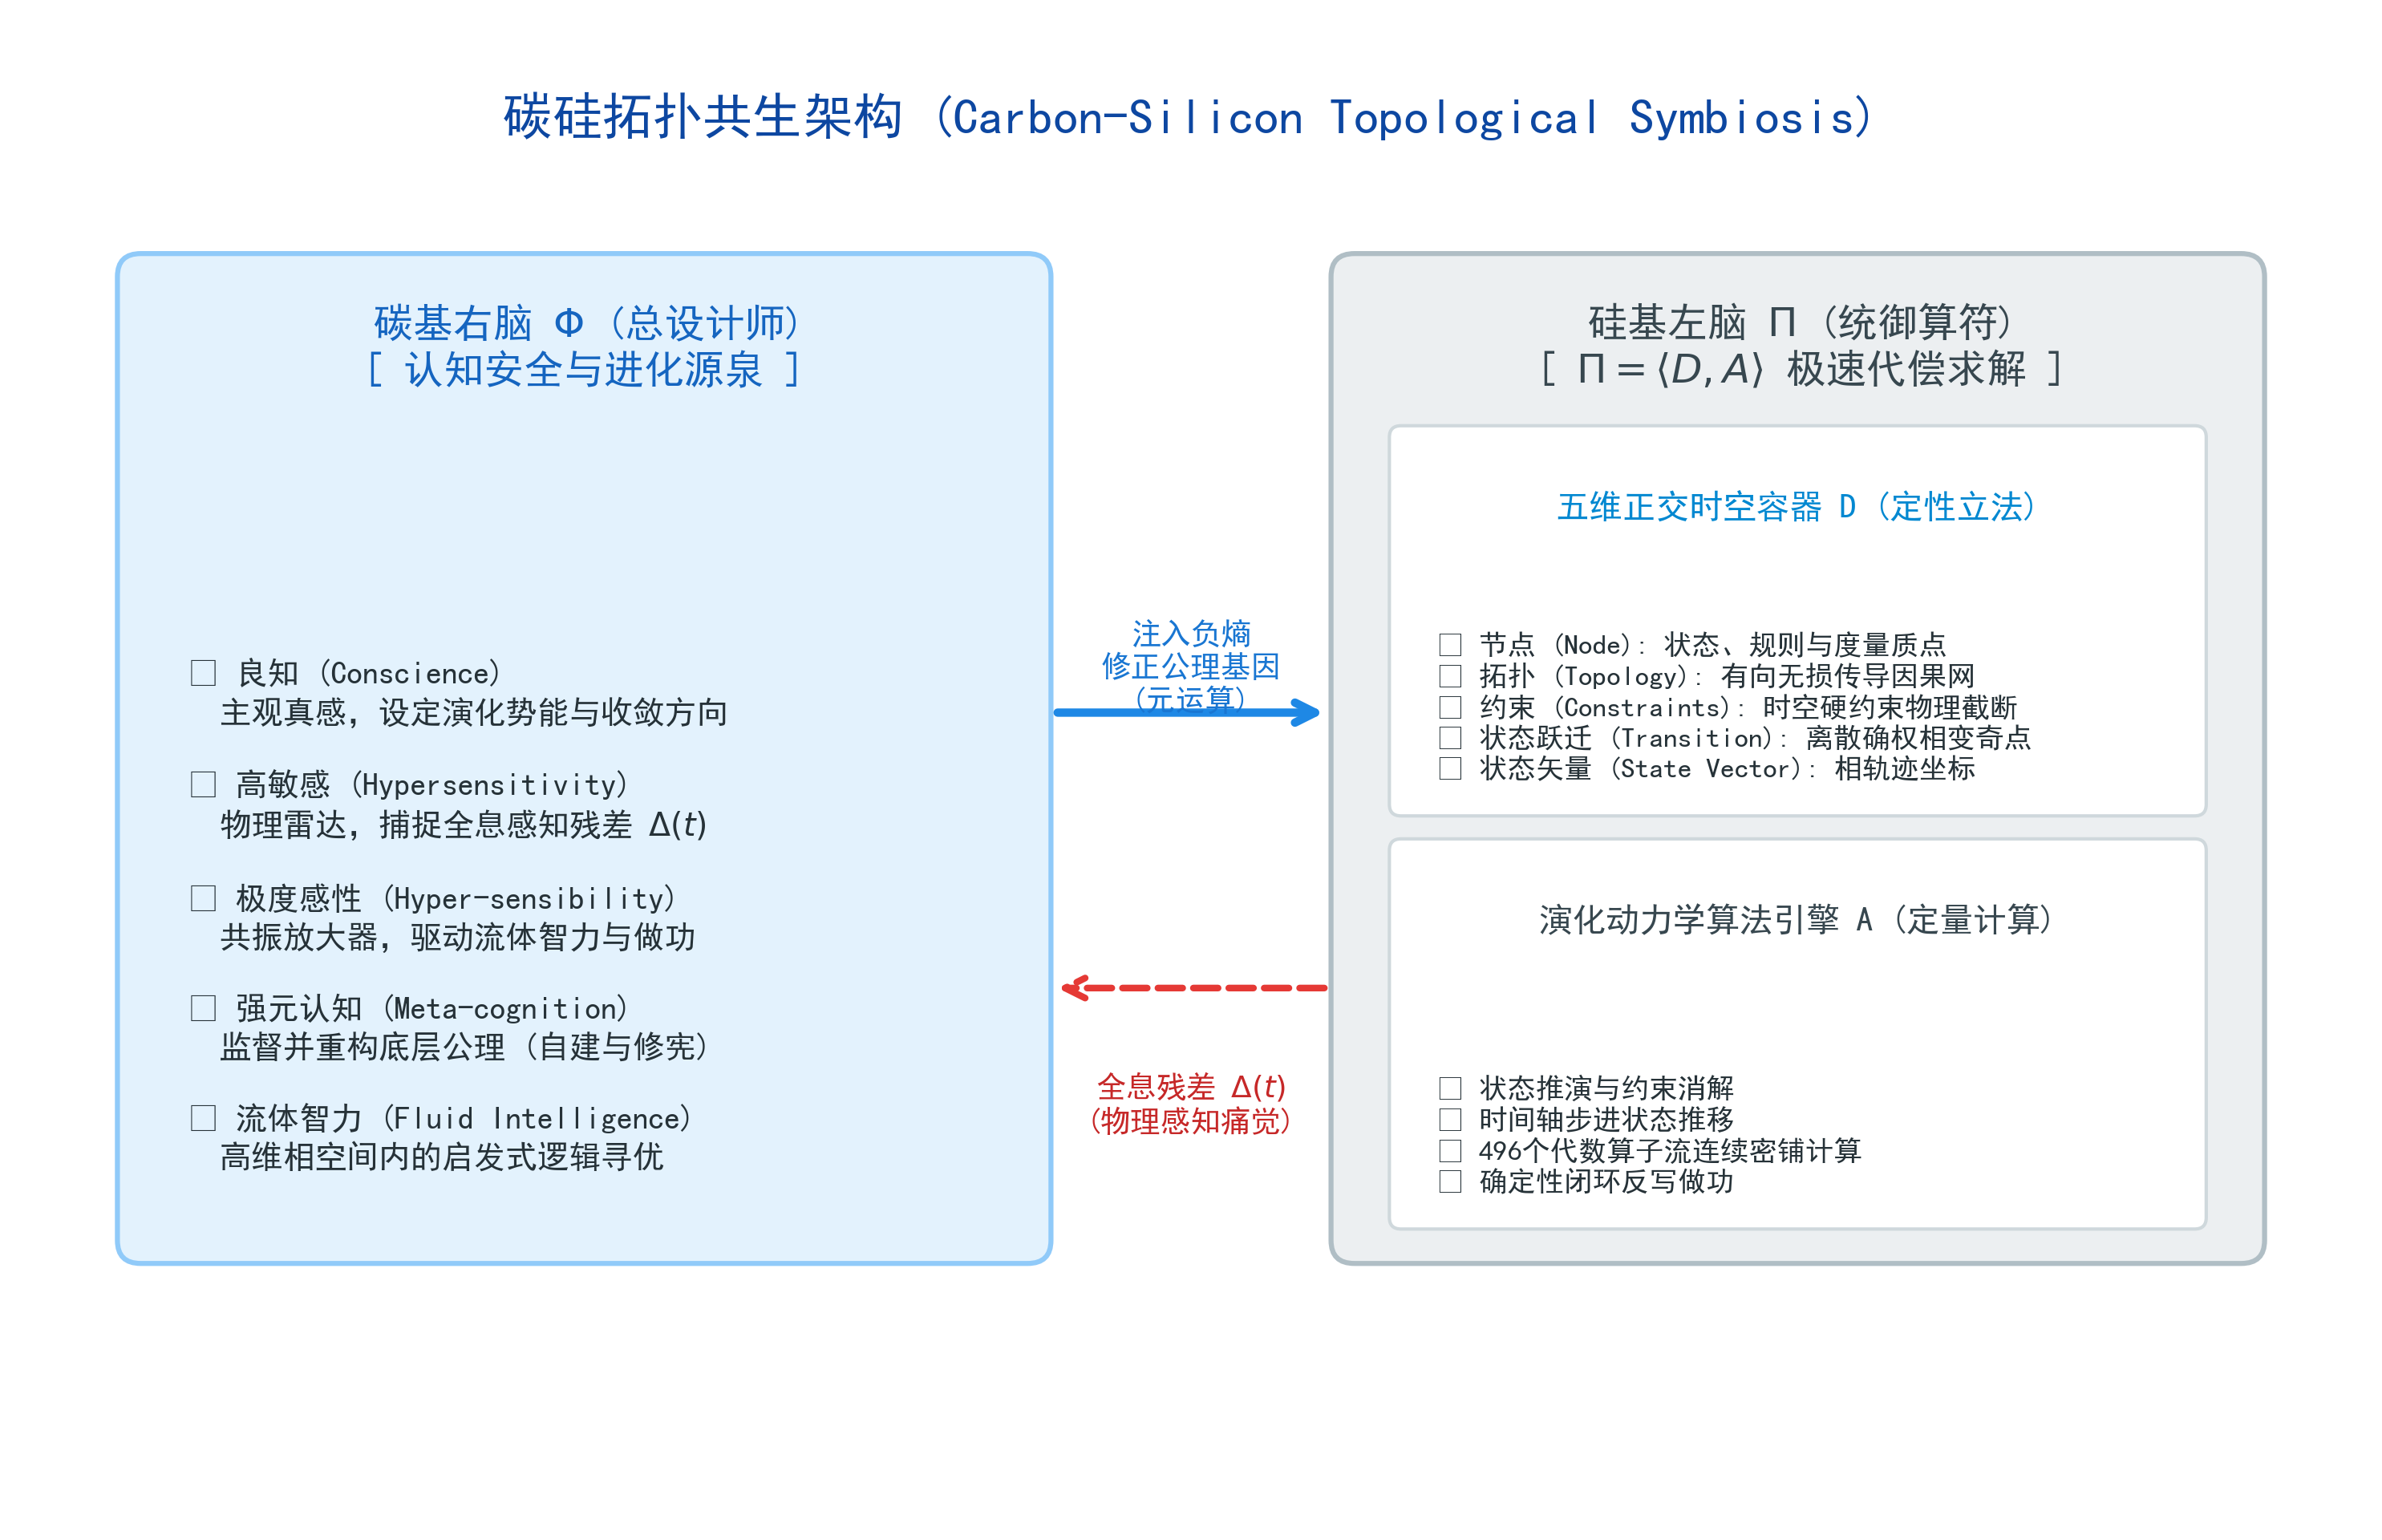
\includegraphics[width=0.85\textwidth]{carbon_silicon_symbiosis.png}
\caption{碳硅拓扑共生架构}
\label{fig:carbon_silicon_symbiosis}
\end{figure}

\subsection*{定理一：综合集成的物理实体是数字双螺旋本体 $\langle D,A \rangle$}
\begin{proof}
根据公理 B，碳基大脑无法处理 $O(N!)$ 级的状态空间，必须引入硅基算符 $\Pi$ 代偿算力极限。根据公理 A，该算符 $\Pi$ 的工程实体是由五维正交时空容器 $D$ 与离散时间步进推演算法 $A$ 深度咬合而成的数字双螺旋。

其中，时空容器 $D$ 被定义为以下五维正交信息流形：
\begin{enumerate}
    \item \textbf{节点 (Node)}：解耦定位系统底层物理、契约与价值实体（解决“主客体是谁”）。
    \item \textbf{拓扑 (Topology)}：定义物质流、契约流、价值流合法转移路径的有向无环图（DAG）及跨维映射矩阵（解决“逻辑结构怎么连”）。
    \item \textbf{约束 (Constraints)}：限制系统相空间自由度的硬性物理边界与柔性契约法理不等式（解决“物理极值边界在哪里”）。
    \item \textbf{状态跃迁 (State Transition)}：物理事件瞬间触发的离散状态变化，执行 1 对 3 的正交投影（解决“动力系统怎么变”）。
    \item \textbf{状态矢量 (State Vector)}：供给势能、需求张力与网络刚度的瞬时动力学快照（解决“系统当前在哪里”）。
\end{enumerate}

该五维正交容器 $D$ 满足严格的 MECE（相互独立，完全穷尽）全息完备性：
\begin{itemize}
    \item \textbf{相互独立 (Mutually Exclusive)}：节点、拓扑、约束、状态跃迁、状态矢量分别描述系统拓扑点、静态连接、解域边界、离散动力变化与瞬时状态坐标，各自由度物理语义互斥，在代数上正交。
    \item \textbf{完全穷尽 (Collectively Exhaustive)}：任何开放自适应系统的状态空间建模，必被完备涵盖为组分拓扑（节点与拓扑）、可行解域（约束）、以及演化轨迹（跃迁与状态矢量）。无论是物理尺度的无机吸积、生物尺度的生存网，还是人类工业价值链，其全息投影无一能脱离此五维表征。
\end{itemize}
由数据模型 $D$ 与业务算法 $A$ 深度咬合而成的 $\langle D,A \rangle$ 闭环运转，在工程上完整实现了“从定性到定量的综合集成”。
\end{proof}

\subsection*{定理二：人机协同是碳基算力代偿与边界突破的双重必然}
\begin{proof}
人机协同的必然性，由两条独立的逻辑支路共同证明：
\begin{itemize}
    \item \textbf{支路一（算力代偿的必然）}：根据公理 B（本质论），碳基大脑的并发信息处理带宽被米勒极限焊死，处于永久算力赤字状态。面对开放复杂巨系统的 $O(N!)$ 级状态空间大爆炸，碳基大脑在物理上无法单独完成全局寻优与实时推演。因此，必须将硅基算符 $\Pi$ 引入系统，作为碳基大脑的算力延伸。硅基负责在既定公理边界内，执行高并发、低时延的定量降维收敛做功；碳基则从算力苦役中解放，回归其不可替代的职能——定义宪法规则与物理边界。此即“硅基代偿，碳基为本”的算力层协同。
    \item \textbf{支路二（边界突破的必然）}：根据公理 C（进化论），任何逻辑自洽的硅基双螺旋系统 $\Pi=\langle D,A \rangle$ 均因哥德尔不完备定理的限制，必然存在其自身无法先验自证并完备涵盖的逻辑死角。当系统撞击该边界时，硅基算符因缺乏处理未知变异的元规则而陷入死锁，系统自发熵增。此时必须引入碳基高阶进化算符 $\Phi$，凭借其痛觉感知残差 $\Delta(t)$，对系统执行变通、物理寻根，并将未知变异重塑为新公理，扩维注入硅基算符。硅基在边界内极速闭环，碳基在边界外自愈进化，此即“碳硅拓扑共生”的进化层协同。
\end{itemize}
\textbf{综合结论}：人机协同的本质是碳基与硅基在算力层（已知规则下的日常做功）与进化层（未知边界上的自我突破）的双重必然结合。其工程实体即为碳硅拓扑共生架构 $\Phi - \Pi$。这一架构在算力维度完整实现了钱老所定义的“人机结合”中硅基代偿的必要性，在进化维度完整实现了“以人为主”中碳基修宪的不可替代性。
\end{proof}

\subsection*{定理三：总设计部是实现“单脑奇点”的必然组织形态}
\begin{proof}
根据公理 A，治理复杂巨系统的双螺旋本体 $\langle D,A \rangle$ 要求业务规则、数据拓扑与求解算法三者深度融合。这三者在认知域上的深度纠缠，必然要求在物质载体上实现同构，即在一个物理大脑（单脑奇点）中同时完成业务解构、数学建模与系统架构的三位一体。根据公理 D，任何试图将此拆解为流水线分工（如业务专家+算法专家+IT架构师）的协作模式，都将因沟通产生的香农信息衰减和 $O(M^2)$ 摩擦内耗而必然失效。因此，必须在组织架构中设立独立的“总设计部实体”并置入具备该三位一体能力的总设计师，以确权全局配额宪法并统御算符架构设计。
\end{proof}

\subsection*{定理四：研讨厅是综合集成与人机协同的工程化产物}
\begin{proof}
由定理一，综合集成的实体是 $\langle D,A \rangle$；由定理二，人机协同的实体是 $\Phi - \Pi$。当碳基总设计师 $\Phi$ 需要干预系统演化时，通过与 $\Pi$ 的交互，在 $D$ 所定义的五维容器内注入新的战略约束，再由 $A$ 在内存中执行超实时推演，将多宇宙平行模拟的结果呈现给 $\Phi$ 进行决策。这种“碳基定方向、硅基跑推演”的高频交互环境，在工程上完整实现了钱老所定义的“从定性到定量综合集成研讨厅”。
\end{proof}

\subsection*{总证：系统具备治理开放复杂巨系统能力的充分必要条件}
\begin{proof}
当且仅当系统采用 $\langle D,A \rangle$ 实现综合集成（定理一），构建 $\Phi - \Pi$ 架构实现人机协同（定理二），设立总设计部实体实现单脑奇点（定理三），并以硅基引擎为内核构建研讨厅（定理四），该系统方具备治理开放复杂巨系统的完整能力。任何违背此架构的系统，均因触犯上述定理所依赖的公理，而在物理与数学上必然走向耗散失效。
这就是对钱老学说的完整形式化证明。
\end{proof}

\section{封疆：从“人治系统”向“无机与有机”群落的大一统分形同构}

全息抗熵理论打破了人类主观社会与自然客观物质的红线，指出一切远离平衡态的自适应自组织系统，其对抗热力学耗散、追求变分自由能最小化的演化轨线，在代数拓扑结构上具有绝对的尺度不变性。

本研究将核心动力学的状态空间大一统投影并收敛至三大层级的超复杂巨系统中：
\begin{enumerate}
    \item \textbf{无机物自组织尺度}：弥散在星际相空间中的尘埃分子云，在自引力势能作用下自发发生向心坍缩、碎裂与多级物质吸积。“全局自引力势能最小化”构成了这一尺度上自然涌现的盲目意志；
    \item \textbf{有机物活跃群落尺度}：群落基质有机物与活性生物质能在食物网拓扑中不可逆流动。在温度与生存压力下，自组织涌现出群落 Flocking 运动，大自然的进化选择压构成了这一尺度上被动的意志；
    \item \textbf{社会与数字工业尺度}：高频变异的千亿级离散制造大盘，子系统投影为研发、营销与交付三大子系统正交解耦后的多维平行流形。由于人类系统无法承受大自然那种高热耗散的被动演化试错，必须由作为观察者
的总设计师主动提炼顶层战略意志向量注入统御算符中。
\end{enumerate}

在跨尺度的拓扑重整中，一切有效抗熵做功均严格遵循变革有效做功标量积方程：
\begin{equation}
    W = \mathbf{F} \cdot \mathbf{S} \cdot \cos \theta
\end{equation}
其中，夹角 $\theta$ 是主观干预矢量与系统客观最优因果轨线之间的错配夹角。系统通过统御算符将微观节点由于盲目碰撞产生的非线性压力向上收敛，彻底消灭由于多重共线性引发的内耗摩擦废热（令 $\theta$ 趋近于 $0$），从而在最底层赋予微观节点在自身轨道内释放动能聚焦做功的绝对自由度。

\section{铸剑：攻克“计算不可约性”与“涌现”大爆炸的工程重剑}

斯蒂芬·沃尔夫勒姆系统阐明了非线性系统的“计算不可约性”：系统演化不可跳步，无法被连续高阶函数精确解析拟合，唯一路径只有一步一步运行。然而，每一步运行背后的离散相空间呈现象级爆炸，是传统数学运筹学的算力天堑。

全息抗熵理论拒绝玄学空谈，直接在千亿级工业极压承压场景下，铸造出了开天辟地的硅基重剑。其核心工程突破，在于对“计算不可约”与“涌现”这对孪生难题的确定性驾驭。

\subsection{计算不可约与涌现：既是问题也是答案}
计算不可约性宣告了任何想用简单公式预测复杂系统未来的企图注定失败——你无法抄近路，你只能一步一步去运行它。而涌现则揭示了，当这不可约的每一步被老老实实执行后，宏观层面的秩序会自发产生，整体大于局部之和。

在工程实践中，这两道物理高墙恰恰指明了唯一正确的路径：不要试图预测涌现，而要设计规则让涌现为你服务；不要试图绕过计算，而要极致优化计算的速度。

本系统的核心算法架构，将复杂的系统逻辑抽象为主干道上有限的关键决策点。即使推演的主干道只有30个核心步骤，每一步计算之后的条件分支，依然会让方案表现出 $2^{30}$ 的超大规模涌现性复杂度。

\begin{proof}[计算不可约下“计算 + 条件分支 (IF-THEN-ELSE) + 再计算”唯一解性证明]
在计算不可约且存在非线性涌现的复杂系统中，步进模拟具有数学上的唯一必然性。
\begin{enumerate}
    \item \textbf{反证支路（不存在解析捷径）}：假设存在某种解析的闭式方程可在不运行系统每一步状态机的前提下，直接计算出未来态的相空间坐标。若该方程存在，则意味着该系统的动力学演化是计算可约的，直接违背了系统具备“计算不可约性”的前置物理公设。因此，解析的捷径在物理上不存在。
    \item \textbf{图灵完备支路（代数表达的唯一性）}：离散相空间的涌现过程等价于图灵机运行。根据邱奇-图灵论题，图灵完备的最小算符集必须包含数据处理（计算）与条件转移（即 \texttt{if-then-else} 分支判断）。在离散计算相空间中，非线性相变与解空间边界切割的唯一代数表达形式，就是基于状态因果的条件转移。
\end{enumerate}
因此，“顺序计算 + 条件分支 (IF-THEN-ELSE) + 再次计算”的步进推演结构，是模拟并求解计算不可约演化过程的唯一合法且必须的数学表达形式。
\end{proof}

正是这种“顺序执行下的非线性相互作用”，使得程序运行的轨迹，就是物理系统在相空间中向最优解自然演化的轨迹。系统不追求一步到位的绝对最优解，而是老老实实地让 CPU 执行“计算 + IF-THEN-ELSE + 再计算”的步进推演。那个最终涌现出的、逻辑自洽且物理可行的结果，就是在当前所有约束下唯一的、确定性的最优解。

\subsection{物理约束代数剪枝}
我们将时间单向性、质能守恒与系统物理极限等物理重力约束直接焊死在 $D$ 容器的最底层。在计算推演极早期直接执行代数截断，强行熔断并过滤掉极大多数没有任何物理执行可能性的泡沫路径，将 NP-hard 相空间的状态大爆炸瞬间降维、压缩为有限状态空间，实现极速收敛。

\subsection{去语义化面向数据设计}
我们彻底摒弃了传统高开销、高延迟的面向对象内存模型，在计算底层设计了去语义化、一维连续紧凑数组与二进制位图向量化计算。它将极为臃肿的系统逻辑直接解构、投影为二进制的 $0$ 和 $1$。利用超导内存计算，消灭了冯·诺依曼架构的传输带宽死锁，在 CPU 高速缓存级实现无锁并发计算。

\subsection{物理物质化闭环做功的判决性实证}
在联宝科技年营收超千亿、80\%以上为5台以下非标碎单的极端离散混合重力场中，本系统在个人笔记本（16核CPU，120G内存，常驻内存计算）上，在5分钟（296秒）以内，彻底收敛并刚性排产了50万笔订单、20层纠缠供应链网络、200万物料大盘的有限产能全局决策。

在推演终点，系统将最优自愈方案一键刚性物质化反写，锁死物理状态分配权。这不是一份“建议书”，它是客观物性重力约束下，底座必须无条件服从的数字秩序。我们用硅基超导计算，强行在时间轴上跑赢了变异，用高频的信息重算，物理代偿了由于人类静态感知产生的系统内耗。

\section{选帅：驾驭开放复杂巨系统的总设计师 L0 级底层认知操作系统}

这套形式化证明与八大物理定律的工程落地，揭示了系统科学最根本、最神圣的碳基内核：大成智慧的奇点总设计师，其心智模型到底是如何在生命演化轨道中坍缩、诞生的？

系统物理学给出了最冷酷的断代判定：总设计师在本质上不是被传统的科层制或教育流水线培养、选拔出来的精英，因为科层制遵循康威定律与局部纳什博弈套利。总设计师是在极限高压的环境中，被体内一种其自己大脑都无法控制的第一性真感觉驱动着，“野蛮”自发生长出来的异类。

这种底层操作系统由五重在世俗眼中具有高度“互斥性”的认知晶格精密咬合而成：
\begin{itemize}
    \item \textbf{良知 (Conscience)}：设定收敛方向。良知并非形而上的道德标榜，而是具身化在总设计师体内的系统引力吸引子势阱，表现为对系统内耗、摩擦与同类受苦的生理性痛觉，为所有的计算与算力设定不容践踏的全局目标函数。
    \item \textbf{高敏感 (Hypersensitivity)}：最前线的物理探针。对客观物理世界与生物节点的感知极度强烈，能瞬间捕捉到被环境噪声遮蔽的微细信号。这是一切认知与痛苦的起点，也是捕捉系统实然与应然间全息残差 $\Delta(t)$ 的物理探针。
    \item \textbf{极度感性 (Hyper-sensibility)}：驱动内核的终极负熵燃料。人类在本质上是预测模型，极度感性让高敏感接收到的信号被深度解码——微观节点遭遇的耗散挣扎，都会在神经镜像系统中产生同频共振，迫使流体智力在相空间开展极限寻优。
    \item \textbf{流体智力 (Fluid Intelligence)}：相空间的寻优引擎。在完全陌生的荒野中，他们不依赖过往经验，利用纯粹推理与模式识别，在面对无先例的复杂网络时，迅速剥离表象语义，抽象出物理本质并执行步进推演。
    \item \textbf{强元认知 (Meta-cognition)}：系统的自指监控与“修宪”算符。不断审视模型与现实的残差，在形式系统面临死锁的奇点，强行打破旧有框架，对公理系统执行拓扑重整与重构。
\end{itemize}

这五项特质极小概率在单个人身上汇聚。他们是逆康威定律、逆科层制的破壁人。

全息抗熵理论对八大定律的形式化证明与代码开源，其终极利他价值，正是为了改良育才土壤，保护脆弱的新一代奇点火种：我们用冰冷、确定的硅基底座，代偿了前人肉身代偿系统断层的痛感，让高敏感、有真感受的杰出者不必每一次都去经历血肉模糊的神经元重塑，而是可以直接手握“八把数字手术刀”，在超导的自洽钢轨上驾驭更广阔的宇宙复杂性。

\section{全息抗熵与系统科学大一统八大定律}

以下八大定律在拓扑代数、测度论与自适应控制论的最高相空间，为整个系统科学宣告了不可逆的形式化主权判决，完备托举、证明了钱学森 OCGS 理论在数智化时代的必然性。

\subsection*{第一定律（目的论）：全域大一统抗熵做功定律}
开放复杂巨系统的自组织存续，本质上是统御算符在非独立同分布的高维张量相空间内注入结构化负熵以对冲系统内生热力学耗散的过程。其动态演化 and 认知闭环受以下三个物理公理共同约束：
\begin{equation}
    dS = d_iS + d_eS \quad \left( d_eS < 0, \; |d_eS| > d_iS \implies dS < 0 \right)
\end{equation}
\begin{equation}
    S_{\text{negative}} = -S = -k_B H(X) = k_B \sum_{i=1}^{n} P(x_i) \log_2 P(x_i)
\end{equation}
\begin{equation}
    F = D_{\text{KL}}\left(q(s) \parallel p(s|o)\right) - \ln p(o) \ge -\ln p(o)
\end{equation}

系统必须以统御（立法）为前置条件，方能闭合“观测、模拟与治理”的因果回路。若缺失统御算符 $\Pi$ 施加的刚性代数约束，系统将陷入闭环反馈辨识死锁与李雅普诺夫时窗天堑：
\begin{equation}
    \text{Cov}(\mathbf{u}, \mathbf{w}) \neq 0 \implies \hat{\theta}_{\text{OLS}} \neq \theta_{\text{true}} \quad (\text{观测不可辨识极限})
\end{equation}
\begin{equation}\label{lyapunov-horizon}
    \tau_{\text{max}} = \frac{1}{\lambda_{\text{max}}} \ln \left( \frac{\Delta_{\text{max}}}{\delta_0} \right) \to 0 \quad (\text{当 } \lambda_{\text{max}} \gg 0 \text{ 时，模拟发散极限})
\end{equation}
无统御状态下，系统最大正李雅普诺夫指数 $\lambda_{\text{max}}$ 呈阶乘级爆炸，导致最大可模拟时窗 $\tau_{\text{max}}$ 坍缩为零，观测空间维度失真，治理做功矢量发生正交对消：
\begin{equation}
    Q = \sum_{i=1}^{n} \|V_i\| - \left\| \sum_{i=1}^{n} V_i \right\| \ge 0 \quad \text{且} \quad W = \mathbf{V}_m \cdot \mathbf{V}_{\pi} \cdot \cos\theta \to 0 \quad (\theta \to 90^\circ)
\end{equation}
因此，必须先通过统御算符 $\Pi$ 设定刚性约束边界，强行将最大李雅普诺夫指数压制至稳定域（$\lambda_{\text{max}} \le 0$），解耦反馈噪声，方能托举全息观测与动态模拟的合法性。

\subsection*{第二定律（本质论）：阿什比极限与硅基代偿定律}
受控系统状态变异数随节点数呈阶乘级爆炸，人类大脑生物学并发信息处理带宽被米勒极限焊死，处于永久算力赤字状态。系统控制力崩溃与机器代偿受以下四重不可约物理定律支配：
\begin{equation}
    V_c \ge V_s \approx O(N!)
\end{equation}
\begin{equation}
    C_{\text{carbon}} = 7 \pm 2 \ll V_s
\end{equation}
\begin{equation}
    \text{Non-IIDness} = f\left(\text{Coupling}(\text{Intra}, \text{Inter}), \text{Heterogeneity}(\text{Dist}, \text{Temp-Spat})\right)
\end{equation}
\begin{equation}
    \max_{p_i} H(X) = -\sum_{i=1}^{n} p_i \ln p_i \quad \text{s.t.} \quad \sum p_i = 1, \; \sum p_i g(x_i) = \bar{G}
\end{equation}
由于实体的非独立同分布性（Non-IIDness）以及高熵状态下的自发最大熵退化，系统的状态空间迅速膨胀至 $O(N!)$。在 $C_{\text{carbon}} \ll V_s$ 的算力塌陷重力下，必须在已知规则边界内，通过在 $D$ 容器最底层强行施加物理极值约束进行代数截断，将控制权无条件、刚性移交至硅基算符 $\Pi$ 以代偿碳基算力极限。

\subsection*{第三定律（方案论）：数字双螺旋本体降维同构定律}
统御中枢在硅基内存中的物理承载是由五维正交容器 $D$ 与离散时间步进推演算法 $A$ 深度耦合而成的数字双螺旋本体。系统在控制论与信息处理上遵循：
\begin{equation}
    \Pi = \langle D, A \rangle : \Omega_{O(N!)} \longrightarrow \Omega_{O(k)}
\end{equation}
\begin{equation}\label{controllability}
    \text{rank}(\mathcal{C}) = \text{rank}\left[ B, AB, A^2B, \dots, A^{n-1}B \right] = n
\end{equation}
\begin{equation}
    h: \Omega \longrightarrow D \quad (\text{Conant-Ashby 同态映射})
\end{equation}
\begin{equation}\label{sampling}
    f_{\text{compute}} > f_{\text{perturbation}} \quad (\text{奈奎斯特采样不等式})
\end{equation}
控制器的算力周转频率 $f_{\text{compute}}$ 必须跑赢外部环境扰动频率 $f_{\text{perturbation}}$。通过全息分形无标度属性（$P(k) \propto k^{-\gamma}$）与可控性满秩约束，在不同层级使用统一的 $\langle D,A \rangle$ 拓扑语法，在内存中吸收 $O(N!)$ 级的状态大爆炸。

\subsection*{第四定律（能力论）：单脑奇点因果逻辑收敛定律}
在多维、非凸硬约束限制下，多个独立行政主体根据阿罗不可能定理，民主拉通在数理上绝对无法加总出全局最优解。跨越复杂性的核心逻辑，在生成期必须强制执行逆康威定律，向同时融通了业务、数据、架构三位一体的“单脑奇点”进行意志坍缩：
\begin{equation}
    \max F(x)_{\text{global}} \neq \sum \max f_i(x)_{\text{local}} \quad \text{且} \quad U_{\text{global}} \neq \sum U_{\text{local}}
\end{equation}
\begin{equation}
    \text{Complexity}_{\text{comm}} = O(K^2) \gg \text{Complexity}_{\text{singularity}} = O(1)
\end{equation}
若引入 $K$ 个节点进行网状决策，通信复杂度将呈 $O(K^2)$ 级爆炸。为了消除信道耗散，必须将全域逻辑强制收敛于单脑奇点，将决策复杂度强行坍缩为 $O(1)$，通过绝对的“逻辑独裁”建立正交的数据基底。

\subsection*{第五定律（机制论）：组织的代数拓扑同构映射定律}
系统数智化转型的协作机制，必须与最终建成的硅基数字大脑运行机制，在数学拓扑上保持分形同构与层级嵌套。系统在宏观涌现与微观分配上遵循贝塔朗菲整体性公式、序参量支配原理与谱分解收敛机制：
\begin{equation}
    V_{\Omega} = f(R) \cdot \sum_{i=1}^{K} V_i \neq \sum_{i=1}^{K} V_i
\end{equation}
\begin{equation}
    V_{\Omega} = M \cdot \Pi \left[ S_1 \otimes S_2 \otimes \dots \otimes S_n \right]
\end{equation}
\begin{equation}
    P = U \Sigma V^T \quad \to \quad P_k = U_k \Sigma_k V_k^T \quad (\text{SVD 谱截断})
\end{equation}
系统通过统御算符 $\Pi$ 在超导内存中将全局协同压力向上收敛重整，消除微观节点 $S_i$ 的跨域协调负担；通过下发重整化后的微观目标与算法（$m_i^*, \pi_i^*$），反向赋予微观节点在特定正交配额边界（Allotment）内聚焦于自身专业轨道做功的绝对自由度。

\subsection*{第六定律（路径论）：维纳-卡尔曼观测边界定律（逆向施工律）}
控制域的维数严格受限于微观观测空间的维度。建设路径必须遵循由底层物理实相向高维形式空间的单向不可逆锚定，满足可观测性条件与罗森建模关系：
\begin{equation}
    \dim \mathcal{C} \le \dim \mathcal{O}
\end{equation}
\begin{equation}
    \text{Encoding} \circ \text{Causal}_{\text{NS}} = \text{Implication}_{\text{FS}} \circ \text{Encoding}
\end{equation}
如果形式系统（FS）计算出的计划解无法通过 Allotment 刚性反写（Decoding / Write-Back）回自然系统（NS）以锁定实物分配权，逻辑就会在物理层悬空。建设路径必须强制执行“逆向物理施工”，先打通执行层探针的编码与反写，方可构筑宏观控制塔。

\subsection*{第七定律（动力论）：行政权力与客观逻辑力场对齐定律}
系统推进加速度与变革实际做功由行政发力与算法引力共同决定，受制于凸优化边界约束与向量标量积定理：
\begin{equation}
    m \cdot \mathbf{a} = \mathbf{F}_M + \mathbf{F}_{\Pi} - \mathbf{f} \quad \text{且} \quad W = \mathbf{V}_m \cdot \mathbf{V}_{\pi} = \|\mathbf{V}_m\| \|\mathbf{V}_{\pi}\| \cos \theta
\end{equation}
\begin{equation}
    \lambda_j = \frac{\partial V_{\Omega}}{\partial b_j}
\end{equation}
系统变革的实际有效做功取决于权力意志矢量 $\mathbf{V}_m$ 与客观技术最优演化轨道 $\mathbf{V}_{\pi}$ 的夹角 $\theta$。统御算符通过解算物理约束边界 $b_j$ 的影子价格（拉格朗日乘子 $\lambda_j$），将行政权力精准倾注于系统瓶颈点，强行收敛夹角令 $\theta \to 0$（即 $\cos\theta \to 1$），实现无损动力做功。

\subsection*{第八定律（进化论）：自适应系统抗热寂进化定律}
静态的硅基公理系统在不完备边界发生逻辑死锁时，必须引入具备“具身良知痛觉”的碳基元认知执行非自回归式公理重写，完成自适应生命体的进化与跃迁：
\begin{equation}
    \frac{dS}{dt} = \frac{d_iS}{dt} + \frac{d_eS}{dt} \quad \left( \frac{d_eS}{dt} < 0, \; \left|\frac{d_eS}{dt}\right| > \frac{d_iS}{dt} \implies \frac{dS}{dt} < 0 \right)
\end{equation}
\begin{equation}\label{evolution-phi}
    \Pi_{t+1} = \Phi\left(\Pi_t, \sum \Delta_{\text{critical}}\right)
\end{equation}
\begin{equation}
    \langle e^{-\beta W} \rangle = e^{-\beta \Delta F} \quad (\text{Jarzynski 非平衡做功等式})
\end{equation}
硅基算符无法自证其逻辑死角。当外部不确定性残差触发系统死锁时，碳基总设计师 $\Phi$ 必须将外界变异残差视为负熵流（$d_eS/dt < 0$）予以吸纳，通过执行物理寻根与算符重构，修改底层公理体系并将未知偏差编译为新的不等式物理约束，完成系统跨代跃迁与碳硅共生自愈。

\section{结论：以智慧为器，以良善为擎}

物理宇宙的耗散重力不包含对人类系统的任何怜悯，孤立的系统在时间的单向铁轨上，终究会自发滑向熵增灭亡的深渊。然而，全息抗熵理论在数理、物理与大脑认知最深处的证明和二十二年的临床实证向世界昭示：

建立全域因果的连接，践行碳硅拓扑的共生，以自身对内外的真切感受（良知）锚定进化的重力，将探索真理、对抗混沌的代码基因代代相传，这就是我们作为高贵的智能生命，在浩瀚、荒凉的热寂宇宙背景下，能够交付给这个世界最大的、最壮丽的逆熵能量。

留在原地的，不再是依赖个别英雄艰难抗争的小作坊，而是一个消除了一切内耗、能够自由呼吸、永续自愈进化的数字生命体。它日夜不息，以最纯粹的理性之光，在这片趋向死寂的宇宙荒漠中，执着地耕耘着一片逆熵的绿洲。

\newpage

\begin{thebibliography}{99}
\bibitem{tsien2001} 钱学森. \emph{创建系统学}[M]. 上海交通大学出版社, 2001.
\bibitem{tsien1990} 钱学森, 于景元, 戴汝为. 一个科学新领域——开放复杂巨系统及其方法论[J]. \emph{自然杂志}, 1990.
\bibitem{fang2011} 方福康. \emph{走向系统科学}[M]. 北京师范大学出版社, 2011.
\bibitem{cao2022} Longbing Cao. Beyond i.i.d.: non-IID thinking, informatics, and learning[J]. \emph{IEEE Intelligent Systems}, 2022.
\bibitem{giuliani2024} Alessandro Giuliani. System Science Can Relax the Tension Between Data and Theory[J]. \emph{Systems}, 2024.
\bibitem{friston2010} Karl Friston. The free-energy principle: a unified brain theory?[J]. \emph{Nature Reviews Neuroscience}, 2010.
\bibitem{sutton2019} Rich Sutton. \emph{The Bitter Lesson}[OL]. LessWrong, 2019.
\bibitem{hoel2025} Erik Hoel. Causal Emergence from Effective Information[J]. \emph{Entropy}, 2025.
\bibitem{el2024} El-Mhamdi El-Mahdi, Lê-Nguyên Hoang. On Goodhart's law, with an application to value alignment[J]. \emph{arXiv preprint}, 2024.
\bibitem{wolfram1987} Stephen Wolfram. Complex Systems and Computational Irreducibility[J]. \emph{Complex Systems}, 1987.
\bibitem{eigen1979} Manfred Eigen. \emph{The Hypercycle: A Principle of Natural Self-Organization}[M]. Springer, 1979.
\bibitem{marblestone2016} Adam Marblestone, Greg Wayne, Konrad Kording. Toward an Integration of Deep Learning and Neuroscience[J]. \emph{Frontiers in Computational Neuroscience}, 2016.
\end{thebibliography}

\end{document}
